\documentclass{article}
\usepackage[margin=0.5in]{geometry}
\usepackage{amsmath}
\usepackage{graphicx}
\usepackage{amssymb}
\usepackage{multicol}
\usepackage{xcolor}
\usepackage{amsthm}
\usepackage{mdframed}

\newenvironment{tightcenter}{%
    \setlength\topsep{0pt}
    \setlength\parskip{0pt}
    \begin{center}
}{%  
    \end{center}
}
\newcommand{\R}{\mathbb{R}}
\newcommand{\Z}{\mathbb{Z}}
\newcommand{\C}{\mathbb{C}}
\newcommand{\K}{\mathbb{K}}
\newcommand{\PP}{\mathbb{P}}
\newcommand{\E}{\mathcal{E}}
\newcommand{\bsum}{\displaystyle\sum}
\title{Trabajo Práctico 2 - Coordenadas, cambio de base, transformaciones lineales I}
\author{Santiago}
\date{}
\begin{document}
    \maketitle
    \global\mdfdefinestyle{s}{%
            linecolor=orange,linewidth=0.5pt,%
            leftmargin=0cm,rightmargin=1cm
        }
    \begin{enumerate}
        \item Sea $B=\{1+x,1+x^2,x+x^2\}$.
    \begin{enumerate}
        \item Probar que $B$ es una base para $\R_2[x]$.
            \begin{mdframed}[style=s]
                Veamos que la única manera de de obtener el polinomio nulo es la trivial.
                \begin{center}
                    $0=\alpha(1+x)+\beta(1+x^2)+\gamma(x+x^2)$\\
                    $\begin{cases}
                        \alpha+\beta=0\\
                        \alpha+\gamma=0\\
                        \beta+\gamma=0
                    \end{cases}\to \alpha=\beta=\gamma=0$
                \end{center}
                Esto indica que los polinomios son linealmente independientes. Además, $\R_2[x]$ es de dimensión 3 y se tienen 3 polinomios li, entonces $B$ genera $\R_2[x]$, por ende, es base.
            \end{mdframed}
        \item Encontrar las coordenadas de $p(x)=3x^2+2x-1$ en la base $B$.
            \begin{mdframed}[style=s]
                \begin{center}
                    $3x^2+2x-1=\alpha(1+x)+\beta(1+x^2)+\gamma(x+x^2)$\\
                    $\begin{cases}
                        \alpha+\beta=-1\\
                        \alpha+\gamma=2\\
                        \beta+\gamma=3
                    \end{cases}\to\begin{cases}
                        \alpha=-1\\
                        \beta=0\\
                        \gamma=3
                    \end{cases}\to[p(x)]_B=\begin{pmatrix}
                        -1\\0\\3
                    \end{pmatrix}$
                \end{center}
            \end{mdframed}
        \item Hallar las coordenadas de los elementos de $B$ en la base canónica de $\R_2[x]$.
            \begin{mdframed}[style=s]
                La base canónica de $\R_2[x]$ es $\E=\{1,x,x^2\}$
                \begin{itemize}
                    \item $1+x=\alpha(1)+\beta(x)+\gamma(x^2)\to[1+x]_\E=\begin{pmatrix}
                            1\\1\\0
                        \end{pmatrix}$
                    \item $1+x^2=\alpha(1)+\beta(x)+\gamma(x^2)\to[1+x^2]_\E=\begin{pmatrix}
                            1\\0\\1
                        \end{pmatrix}$
                    \item $x+x^2=\alpha(1)+\beta(x)+\gamma(x^2)\to[x+x^2]_\E=\begin{pmatrix}
                            0\\1\\1
                        \end{pmatrix}$
                \end{itemize}
            \end{mdframed}
        \item Escribir a los vectores de la base canónica de $\R_2[x]$ como combinación lineal de los elementos de $B$
            \begin{mdframed}[style=s]
                \begin{itemize}
                    \item $1=\alpha(1+x)+\beta(1+x^2)+\gamma(x+x^2)\to[1]_B=\begin{pmatrix}
                            1/2\\1/2\\-1/2
                        \end{pmatrix}$
                    \item $x=\alpha(1+x)+\beta(1+x^2)+\gamma(x+x^2)\to[x]_B=\begin{pmatrix}
                            1/2\\-1/2\\1/2
                        \end{pmatrix}$
                    \item $x^2=\alpha(1+x)+\beta(1+x^2)+\gamma(x+x^2)\to[x^2]_B=\begin{pmatrix}
                            -1/2\\1/2\\1/2
                        \end{pmatrix}$
                \end{itemize}
            \end{mdframed}
    \end{enumerate}
        \item Sean $\E$ la base canónica de $\R^3$ y $B=\{(1,1,0);(1,1,1);(0,1,1)\}$.
    \begin{enumerate}
        \item Hallar la matriz $P_{\E,B}$ de cambio de base de $B$ en $\E$.
            \begin{mdframed}[style=s]
                \begin{center}
                    $P_{\E,B}=\left([(1,1,0)]_\E\quad[(1,1,1)]_\E\quad[(0,1,1)]_\E\right)$\\
                    $P_{\E,B}=\begin{pmatrix}
                        1&1&0\\1&1&1\\0&1&1
                    \end{pmatrix}$
                \end{center}
                En la Figura 1 se muestra como $[g]_B=\begin{pmatrix}
                    1&1&0
                \end{pmatrix}^T$, es escrito en términos de la base canónica.($[g]_\E=P_{\E,B}\cdot[g]_B=\begin{pmatrix}
                    2&2&1
                \end{pmatrix}^T$)
                \begin{center}
                    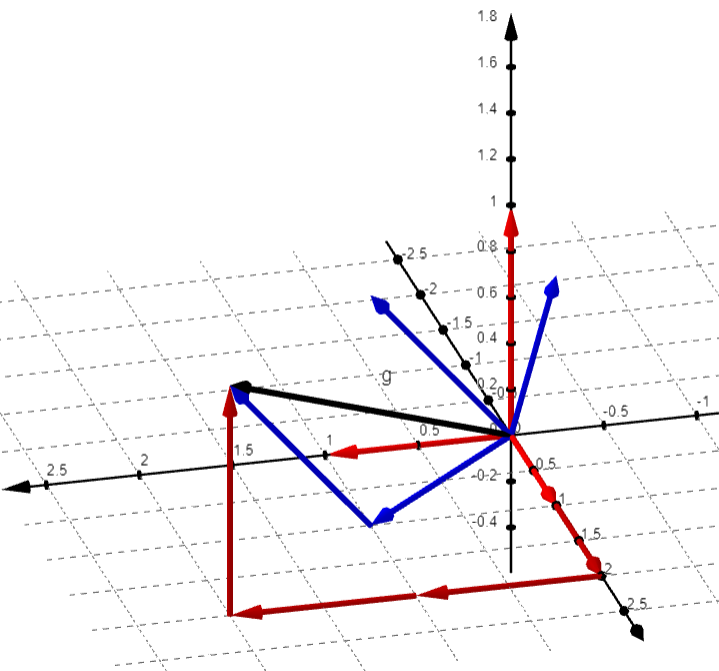
\includegraphics[width=0.4\textwidth]{img/Ej2a.png}\\
                    Figura 1. Vector g representado en dos bases diferentes.
                \end{center}
            \end{mdframed}
        \item Hallar la matriz $P_{B,\E}$ de cambio de base de $\E$ en $B$.
            \begin{mdframed}[style=s]
                \begin{center}
                    $P_{B,\E}=\left([(1,0,0)]_B\quad[(0,0,0)]_B\quad[(0,0,1)]_B\right)$\\
                    $P_{B,\E}=\begin{pmatrix}
                        0&1&-1\\1&-1&1\\-1&1&0
                    \end{pmatrix}$
                \end{center}
            \end{mdframed}
        \item Comprobar que la matriz hallada en el ítem $a)$ es la inversa de la del ítem $b)$.
            \begin{mdframed}[style=s]
                Para que sean inversas, su producto tiene que dar como resultado la matriz identidad:
                \begin{center}
                    $\begin{pmatrix}
                        1&1&0\\1&1&1\\0&1&1
                    \end{pmatrix}\cdot\begin{pmatrix}
                        0&1&-1\\1&-1&1\\-1&1&0
                    \end{pmatrix}=\begin{pmatrix}
                        1&0&0\\0&1&0\\0&0&1
                    \end{pmatrix}$
                \end{center}
            \end{mdframed}
        \item Comprobar que $P_{B,\E}[(1,2,0)]_\E=[(1,2,0)]_B$.
            \begin{mdframed}[style=s]
                Una forma sería:
                \begin{align*}
                    P_{B,\E}[(1,2,0)]_\E&=[(1,2,0)]_B\\
                    P_{B,\E}P_{\E,B}[(1,2,0)]_B&=[(1,2,0)]_B\\
                    I[(1,2,0)]_B&=[(1,2,0)]_B\\
                    [(1,2,0)]_B&=[(1,2,0)]_B
                \end{align*}
                Mientras que también se puede:
                \begin{center}
                    $\begin{pmatrix}
                        0&1&-1\\1&-1&1\\-1&1&0
                    \end{pmatrix}[(1,2,0)]_\E=\begin{pmatrix}
                        0&1&-1\\1&-1&1\\-1&1&0
                    \end{pmatrix}\cdot\begin{pmatrix}
                        1\\2\\0
                    \end{pmatrix}=\begin{pmatrix}
                        2\\-1\\1
                    \end{pmatrix}$
                \end{center}
                y ahora resta encontrar $[(1,2,0)]_B,\quad(1,2,0)=\alpha(1,1,0)+\beta(1,1,1)+\gamma(0,1,1)$
                \begin{center}
                    $\begin{cases}
                        1=\alpha+\beta\\
                        2=\alpha+\beta+\gamma\\
                        0=\beta+\gamma
                    \end{cases}\to\begin{cases}
                        \alpha=2\\
                        \beta=-1\\
                        \gamma=1
                    \end{cases}$
                \end{center}
                Lo cual coincide con el resultado previo.
            \end{mdframed}
    \end{enumerate}
        \item Sea $\E=\{e_1,\dots,e_n\}$ la base canónica de $\R^n$(como $\R$-EV) y sean
    \begin{center}
        $u_1=e_2-e_1,$ $ u_2=e_3-e_2,\dots,u_{n-1}=e_n-e_{n-1},$ $u_n=e_n$ 
    \end{center}
    \begin{enumerate}
        \item Probar que $B=\{u_1,\dots,u_n\}$ es una base de $\R^n$.
            \begin{mdframed}[style=s]
                $B$ tiene $n$ elementos, así que si muestro que son li, entonces es base.
                \begin{align*}
                    0&=\displaystyle\sum_{i=1}^nx_iu_i=\bsum_{i=1}^{n-1}x_i(e_{i+1}-e_i)+x_ne_n\\
                    &=x_1e_2+x_2e_3+x_3e_4+\dots+x_{n-1}e_n\\
                    -x_1e_1&-x_2e_2-x_3e_3-x_4e_4-\dots-x_{n-1}e_{n-1}+x_ne_n\\
                    &=(-x_1)e_1+(x_1-x_2)e_2+(x_2-x_3)e_3+\dots+(x_{n-2}-x_{n-1})e_{n-1}+(x_{n-1}+x_n)e_n
                \end{align*}
                Se ve que $0$ quedó expresado como combinación lineal de los vectores de la base canónica. Como estos son li, todos los escalares deben ser $0$. Por lo tanto
                \begin{center}
                    $-x_1=(x_1-x_2)=(x_2-x_3)=\dots=(x_{n-2}-x_{n-1})=(x_{n-1}+x_n)=0$\\
                    $\to x_1=x_2=x_3=\dots=x_{n-1}=x_n=0$
                \end{center}
                Entonces, la única manera de obtener el vector nulo como combinación lineal de los vectores de $B$ es con escalares nulos, entonces $B$ es un conjunto li.\vspace{6pt}\\
                Otra manera de verificar que sean li, hubiese sido armando una matriz cuyas columnas sean los vectores de $B$ y calcular su determinante. Tenemos que
                \begin{align*}
                    u_1&=(-1,1,0,0,\dots,0,0)\\
                    u_2&=(0,-1,1,0,\dots,0,0)\\
                    u_3&=(0,0,-1,1,\dots,0,0)\\
                    &\vdots\\
                    u_{n-1}&=(0,0,0,0,\dots,-1,1)\\
                    u_n&=(0,0,0,0,\cdots,0,1)
                \end{align*}
                Al ponerlo en forma de matriz:
                \begin{center}
                    $\begin{pmatrix}
                        -1&0&0&\dots&0&0\\
                        1&-1&0&\dots&0&0\\
                        0&1&-1&\dots&0&0\\
                        &\vdots&&&\vdots&\\
                        0&0&0&\dots&-1&0\\
                        0&0&0&\dots&1&1
                    \end{pmatrix}$
                \end{center}
                Se ve que como resultado tengo una matriz triangular. Entonces el determinante es $(-1)^{n-1}\neq 0$. Por lo tanto, los vectores $u_i\in B$ son li.
            \end{mdframed}
        \item Hallar las matrices de cambio de base $P_{\E,B}$ y $P_{B,\E}$ para $n=3$.
            \begin{mdframed}[style=s]
                Para $n=3$: $\E=\{(1,0,0);(0,1,0);(0,0,1)\}$ y $B=\{(-1,1,0);(0,-1,1);(0,0,1)\}$
                \begin{align*}
                    P_{\E,B}=\left([(-1,1,0)]_\E\quad[(0,-1,1)]_\E\quad[(0,0,1)]_\E\right)&=\begin{pmatrix}
                        -1&0&0\\1&-1&0\\0&1&1
                    \end{pmatrix}\\
                    P_{B,\E}=\left([(1,0,0)]_B\quad[(0,1,0)]_B\quad[(0,0,1)]_B\right)&=\begin{pmatrix}
                        -1&0&0\\-1&-1&0\\1&1&1
                    \end{pmatrix}
                \end{align*}
            \end{mdframed}
        \item Probar que para todo $v\in\R^3$, se tiene que $[v]_B=P_{B,\E}[v]_\E$.
            \begin{mdframed}[style=s]
                Sea $v\in\R^3\to$
                \begin{center}
                    $v=(x,y,z)=\alpha(-1,1,0)+\beta(0,-1,1)+\gamma(0,0,1)$\\
                    $\begin{cases}
                        x=-\alpha\\
                        y=\alpha-\beta\\
                        z=\beta+\gamma
                    \end{cases}\to\begin{cases}
                        \alpha=-x\\
                        \beta=-x-y\\
                        \gamma=x+y+z
                    \end{cases}$\\
                    $\to v=(-x)(-1,1,0)+(-x-y)(0,-1,1)+(x+y+z)(0,0,1)$\\
                    $\to [v]_B=\begin{pmatrix}
                        -x\\-x-y\\x+y+z
                    \end{pmatrix}$
                \end{center}
                Por otra parte,
                \begin{center}
                    $P_{B,\E}[v]_\E=\begin{pmatrix}
                        -1&0&0\\-1&-1&0\\1&1&1
                    \end{pmatrix}\cdot\begin{pmatrix}
                        x\\y\\z
                    \end{pmatrix}=\begin{pmatrix}
                        -x\\-x-y\\x+y+z
                    \end{pmatrix}$
                \end{center}
                Y se ve que ambos resultados son iguales.
            \end{mdframed}
    \end{enumerate}
        \item \begin{enumerate}
        \item Hallar una base de $\C_3[x]$ que no sea la canónica.
            \begin{mdframed}[style=s]
                Propongo $B_1=\{1,x,x^2+1,x^3\}$. Para verificar que sea una base, me fijo si los polinomios son li.
                \begin{center}
                    $0=\alpha+\beta x+\gamma (x^2+1)+\delta x^3\to\begin{cases}
                        \alpha+\gamma=0\\
                        \beta=0\\
                        \gamma=0\\
                        \delta=0
                    \end{cases}\to\alpha=0$
                \end{center}
                Al tener 4 polinomios li, estos generan $\C_3[x]$ y por ende son base.
            \end{mdframed}
        \item Hallar la matriz de cambio de base de $B=\{1-x,x-x^2,x^2-x^3,x^3\}$ en la base hallada en el ítem anterior.
            \begin{mdframed}[style=s]
                \begin{center}
                    $P_{B_1,B}=\left([1-x]_{B_1}\quad[x-x^2]_{B_1}\quad[x^2-x^3]_{B_1}\quad[x^3]_{B_1}\right)$\\
                    $P_{B_1,B}=\begin{pmatrix}
                        1&1&-1&0\\-1&1&0&0\\0&-1&1&0\\0&0&-1&1
                    \end{pmatrix}$
                \end{center}
            \end{mdframed}
        \item ¿Cuáles son las coordenadas de $3x^3-x+2$ en la base $B$?
            \begin{mdframed}[style=s]
                \begin{center}
                    $P_{B,\E}=\left([1]_{B}\quad[x]_{B}\quad[x^2]_{B}\quad[x^3]_{B}\right)$\\
                    $P_{B,\E}=\begin{pmatrix}
                        1&0&0&0\\1&1&0&0\\1&1&1&0\\1&1&1&1
                    \end{pmatrix}$\\
                    $\to [3x^3-x+2]_B=P_{B,\E}[3x^3-x+2]_\E$\\
                    $\to[3x^3-x+2]_B=\begin{pmatrix}
                        1&0&0&0\\1&1&0&0\\1&1&1&0\\1&1&1&1
                    \end{pmatrix}\cdot\begin{pmatrix}
                        2\\-1\\0\\3
                    \end{pmatrix}=\begin{pmatrix}
                        2\\1\\1\\4
                    \end{pmatrix}$
                \end{center}
            \end{mdframed}
    \end{enumerate}
        \item Considerar los siguientes subconjuntos de $\R^{2\times2}$.
    \begin{itemize}
        \item $B_1=\left\{\begin{pmatrix}
                1&0\\1&0
            \end{pmatrix};\begin{pmatrix}
                1&1\\0&0
            \end{pmatrix};\begin{pmatrix}
                1&1\\1&0
            \end{pmatrix};\begin{pmatrix}
                0&0\\0&1
            \end{pmatrix}\right\}$.
        \item $B_2=\left\{\begin{pmatrix}
                -1&0\\1&-1
            \end{pmatrix};\begin{pmatrix}
                0&0\\0&-1
            \end{pmatrix};\begin{pmatrix}
                -1&1\\0&1
            \end{pmatrix};\begin{pmatrix}
                1&0\\0&0
            \end{pmatrix}\right\}$.
    \end{itemize}
    \begin{enumerate}
        \item Probar que $B_1$ y $B_2$ son bases para $\R^{2\times2}$.
            \begin{mdframed}[style=s]
                Nuevamente hay que verificar que sean li.
                \begin{itemize}
                    \item $\begin{pmatrix}
                            0&0\\0&0
                        \end{pmatrix}=x_1\begin{pmatrix}
                            1&0\\1&0
                        \end{pmatrix}+x_2\begin{pmatrix}
                            1&1\\0&0
                        \end{pmatrix}+x_3\begin{pmatrix}
                            1&1\\1&0
                        \end{pmatrix}+x_4\begin{pmatrix}
                            0&0\\0&1
                        \end{pmatrix}\to\begin{cases}
                            x_1+x_2+x_3=0\\
                            x_2+x_3=0\\
                            x_1+x_3=0\\
                            x_4=0
                        \end{cases}$
                        \begin{center}
                            $\to x_1=x_2=x_3=x_4=0$    
                        \end{center}
                        Por ende, $B_1$ es base.
                    \item $\begin{pmatrix}
                            0&0\\0&0
                        \end{pmatrix}=x_1\begin{pmatrix}
                            -1&0\\1&-1
                        \end{pmatrix}+x_2\begin{pmatrix}
                            0&0\\0&-1
                        \end{pmatrix}+x_3\begin{pmatrix}
                            -1&1\\0&1
                        \end{pmatrix}+x_4\begin{pmatrix}
                            1&0\\0&0
                        \end{pmatrix}\to\begin{cases}
                            -x_1-x_3+x_4=0\\
                            x_3=0\\
                            x_1=0\\
                            -x_1-x_2+x_3=0
                        \end{cases}$
                        \begin{center}
                            $\to x_1=x_2=x_3=x_4=0$
                        \end{center}
                        Por lo tanto, $B_2$ es base.
                \end{itemize}
            \end{mdframed}
        \item Hallar la matriz de cambio de base de $B_2$ en la base $B_1$.
            \begin{mdframed}[style=s]
                \begin{center}
                    $P_{B_1,B_2}=\left(\left[\begin{pmatrix}
                        -1&0\\1&-1
                    \end{pmatrix}\right]_{B_1}\quad\left[\begin{pmatrix}
                        0&0\\0&-1
                    \end{pmatrix}\right]_{B_1}\quad\left[\begin{pmatrix}
                        -1&1\\0&1
                    \end{pmatrix}\right]_{B_1}\quad\left[\begin{pmatrix}
                        1&0\\0&0
                    \end{pmatrix}\right]_{B_1}\right)$
                \end{center}
                Para saber las coordenadas de una matriz arbitraria en la base $B_1$, podemos plantear
                \begin{center}
                    $\begin{pmatrix}
                        a&b\\c&d
                    \end{pmatrix}=x_1\begin{pmatrix}
                        1&0\\1&0
                    \end{pmatrix}+x_2\begin{pmatrix}
                        1&1\\0&0
                    \end{pmatrix}+x_3\begin{pmatrix}
                        1&1\\1&0
                    \end{pmatrix}+x_4\begin{pmatrix}
                        0&0\\0&1
                    \end{pmatrix}$\\
                    $\to \begin{cases}
                        a=x_1+x_2+x_3\\
                        b=x_2+x_3\\
                        c=x_1+x_3\\
                        d=x_4
                    \end{cases}\to\begin{cases}
                        x_1=a-b\\
                        x_2=a-c\\
                        x_3=-a+b+c\\
                        x_4=d
                    \end{cases}$\\
                    $P_{B_1,B_2}=\begin{pmatrix}
                        -1-0&0-0&-1-1&1-0\\-1-1&0-0&-1-0&1-0\\-(-1)+0+1&-0+0+0&-(-1)+1+0&-1+0+0\\-1&-1&1&0
                    \end{pmatrix}=\begin{pmatrix}
                        -1&0&-2&1\\-2&0&-1&1\\2&0&2&-1\\-1&-1&1&0
                    \end{pmatrix}$
                \end{center}
            \end{mdframed}
        \item ¿Cuáles son las coordenadas de $\begin{pmatrix}
                0&1\\1&-2
            \end{pmatrix}$ en la base $B_2$?¿Y en la base $B_1$?
            \begin{mdframed}[style=s]
                Para la base $B_1$ en el inciso anterior obtuve los escalares en base a las entradas de la matriz
                \begin{center}
                    $\to\left[\begin{pmatrix}
                        0&1\\1&-2
                    \end{pmatrix}\right]_{B_1}=\begin{pmatrix}
                        -1\\-1\\2\\-2
                    \end{pmatrix}$
                \end{center}
                Para tener las coordenadas en la base $B_2$, puedo encontrar la matriz de cambio de base de $\E$ a $B_2$:
                \begin{center}
                    $P_{B_2,\E}=\left([E_1]_{B_2}\quad[E_2]_{B_2}\quad[E_3]_{B_2}\quad[E_4]_{B_2}\right)$\\
                    $P_{B_2,\E}=\begin{pmatrix}
                        0&0&1&0\\0&1&-1&-1\\0&1&0&0\\1&1&1&0
                    \end{pmatrix}$\\
                    $\left[\begin{pmatrix}
                        0&1\\1&-2
                    \end{pmatrix}\right]_{B_2}=\begin{pmatrix}
                        0&0&1&0\\0&1&-1&-1\\0&1&0&0\\1&1&1&0
                    \end{pmatrix}\cdot\begin{pmatrix}
                        0\\1\\1\\-2
                    \end{pmatrix}=\begin{pmatrix}
                        1\\2\\1\\2
                    \end{pmatrix}$
                \end{center}
                Ahora podemos comprobar con la matriz del inciso anterior
                \begin{center}
                    $\left[\begin{pmatrix}
                        0&1\\1&-2
                    \end{pmatrix}\right]_{B_1}=P_{B_2,B_1}\cdot\left[\begin{pmatrix}
                        0&1\\1&-2
                    \end{pmatrix}\right]_{B_2}=\begin{pmatrix}
                        -1&0&-2&1\\-2&0&-1&1\\2&0&2&-1\\-1&-1&1&0
                    \end{pmatrix}\cdot\begin{pmatrix}
                        1\\2\\1\\2
                    \end{pmatrix}=\begin{pmatrix}
                        -1\\-1\\2\\-2
                    \end{pmatrix}$
                \end{center}
            \end{mdframed}
    \end{enumerate}
        \item Hallar las matrices de cambio de base $P_{B_1,B_2}$ y $P_{B_2,B_1}$ para cada uno de los siguientes casos.
    \begin{enumerate}
        \item En $\R^3, B_1=\{(5,3,1);(1,-3,-2);(1,2,1)\}$ y $B_2=\{(-2,1,0);(-1,-3,0);(-2,-3,1)\}$
            \begin{mdframed}[style=s]
                Empiezo con $P_{B_2,B_1}$, la matriz de cambio de base de $B_1$ a $B_2$. Una forma que se me ocurre es la siguiente. Si tenemos un vector $v$ representado en las coordenadas de la base $B_1$, \[[v]_{B_1}=\begin{pmatrix}
                    a\\b\\c
                \end{pmatrix}\quad a,b,c\in\R\]Es decir que \[v=a(5,3,1)+b(1,-3,-2)+c(1,2,1)\]
                Por otra parte, $v$ también puede ser representado en términos de la base $B_2$\[[v]_{B_2}=\begin{pmatrix}
                    d\\e\\f
                \end{pmatrix}\quad d,e,f\in\R\]
                Entonces,\[v=d(-2,1,0)+e(-1,-3,0)+f(-2,-3,1)\]Por lo tanto tenemos que,\[a(5,3,1)+b(1,-3,-2)+c(1,2,1)=d(-2,1,0)+e(-1,-3,0)+f(-2,-3,1)\]De donde obtenemos el siguiente sistema de ecuaciones:
                \begin{center}
                    $\begin{cases}
                        5a+b+c=-2d-e-2f\\
                        3a-3b+2c=d-3e-3f\\
                        a-2b+c=f
                    \end{cases}$
                \end{center}
                Resolviendo para $d,e$ y $f$, llegamos a
                \begin{center}
                    $\begin{cases}
                        d=(-15a-4c)/7\\
                        e=(-19a+21b-13c)/7\\
                        f=a-2b+c
                    \end{cases}\to [v]_{B_2}=\begin{pmatrix}
                        (-15a-4c)/7\\
                        (-19a+21b-13c)/7\\
                        a-2b+c
                    \end{pmatrix}$
                \end{center}
                El objetivo es obtener la matriz de cambio de base, osea necesitamos que se cumpla\[\begin{pmatrix}
                    (-15a-4c)/7\\
                    (-19a+21b-13c)/7\\
                    a-2b+c
                \end{pmatrix}=P_{B_2,B_1}\cdot \begin{pmatrix}
                    a\\b\\c
                \end{pmatrix}\]Por lo tanto,\[P_{B_2,B_1}=\begin{pmatrix}
                    -15/7&0&-4/7\\-19/7&3&-13/7\\1&-2&1
                \end{pmatrix}\]
                Para hallar $P_{B_1,B_2}$ calculamos $P_{B_2,B_1}^{-1}$\[P_{B_1,B_2}=\begin{pmatrix}
                    -5&8&12\\
                    6&-11&-17\\
                    17&-30&-45                   
                \end{pmatrix}\]
            \end{mdframed}
        \item En $\C_3[x], B_1=\{1,x-1,x^2-x,x^3\}$ y $B_2=\{x,x-1,x^2,x^3+1\}$
            \begin{mdframed}[style=s]
                En este caso, podría hacer el mismo procedimiento que antes, pero para variar un poco:\[P_{B_1,B_2}=\left([x]_{B_1}\quad[x-1]_{B_1}\quad[x^2]_{B_1}\quad[x^3+1]_{B_1}\right)\]\begin{center}
                    $\begin{cases}
                        x&=a_1(1)+b_1(x-1)+c_1(x^2-x)+d_1(x^3)\\
                        x-1&=a_2(1)+b_2(x-1)+c_2(x^2-x)+d_2(x^3)\\
                        x^2&=a_3(1)+b_3(x-1)+c_3(x^2-x)+d_3(x^3)\\
                        x^3+1&=a_4(1)+b_4(x-1)+c_4(x^2-x)+d_4(x^3)
                    \end{cases}\to\begin{cases}
                        a_1=1,b_1=1,c_1=0,d_1=0\\
                        a_2=0,b_2=1,c_2=0,d_2=0\\
                        a_3=1,b_3=1,c_3=1,d_3=0\\
                        a_4=1,b_4=0,c_4=0,d_4=1
                    \end{cases}$\\
                    $P_{B_1,B_2}=\begin{pmatrix}
                        1&0&1&1\\1&1&1&0\\0&0&1&0\\0&0&0&1
                    \end{pmatrix}$
                \end{center}
                Con la inversa obtengo:\[P_{B_2,B_1}=\begin{pmatrix}
                    1 &0&-1&-1\\
                    -1&1&0 & 1\\
                    0 &0&1 & 0\\
                    0 &0&0 & 1
                \end{pmatrix}\]
            \end{mdframed}
    \end{enumerate}
        \item Sea $B_1=\{(1,0,1);(1,1,0);(0,0,1)\}$ una base de $\R^3$. Si
    \begin{center}
        $P_{B_2,B_1}=\begin{pmatrix}
            1&1&2\\2&1&1\\-1&-1&1
        \end{pmatrix}$.
    \end{center}
    Hallar los vectores de la base $B_2$.
    \begin{mdframed}[style=s]
        \[P_{B_2,B_1}=\left([(1,0,1)]_{B_2}\quad[(1,1,0)]_{B_2}\quad[(0,0,1)]_{B_2}\right)\]
        Osea que\[[(1,0,1)]_{B_2}=\begin{pmatrix}
            1\\2\\-1
        \end{pmatrix}\quad[(1,1,0)]_{B_2}=\begin{pmatrix}
            1\\1\\-1
        \end{pmatrix}\quad[(0,0,1)]_{B_2}=\begin{pmatrix}
            2\\1\\1
        \end{pmatrix}\]Entonces\begin{center}
            $\begin{cases}
                (1,0,1)=1v_1+2v_2-1v_3\\
                (1,1,0)=1v_1+1v_2-1v_3\\
                (0,0,1)=2v_1+1v_2+1v_3
            \end{cases}$
        \end{center}
        siendo $B_2=\{v_1,v_2,v_3\}$. Si $v_i=(v_{ix},v_{iy},v_{iz})\quad i=1,2,3\to$
        \begin{center}
            $\begin{cases}
                1=v_{1x}+2v_{2x}-v_{3x}\\
                1=v_{1x}+v_{2x}-v_{3x}\\
                0=2v_{1x}+v_{2x}+v_{3x}\\
            \end{cases},\quad\begin{cases}
                0=v_{1y}+2v_{2y}-v_{3y}\\
                1=v_{1y}+v_{2y}-v_{3y}\\
                0=2v_{1y}+v_{2y}+v_{3y}\\
            \end{cases},\quad\begin{cases}
                1=v_{1z}+2v_{2z}-v_{3z}\\
                0=v_{1z}+v_{2z}-v_{3z}\\
                1=2v_{1z}+v_{2z}+v_{3z}\\
            \end{cases}$
        \end{center}
        De donde se obtiene que \[v_1=\begin{pmatrix}
            1/3\\1\\-1/3
        \end{pmatrix},\quad v_2=\begin{pmatrix}
            0\\-1\\1
        \end{pmatrix},\quad v_3=\begin{pmatrix}
            -2/3\\-1\\2/3
        \end{pmatrix}\]
    \end{mdframed}
        \item Determinar si las siguientes aplicaciones son transformaciones lineales.
    \begin{enumerate}
        \item $T:\R^3\to\R^3$ dada por $T(x,y,z)=(x-y,x^2,2z)$.
            \begin{mdframed}[style=s]
                Para que una aplicación $T:V\to W$ sea una transformación lineal se deben cumplir dos cosas:
                \begin{enumerate}
                    \item $T(a+b)=T(a)+T(b)\quad \forall a,b\in V$
                    \item $T(\alpha a)=\alpha T(a)\quad\forall \alpha\in\K,a\in V$
                \end{enumerate}
                También se pueden combinar ambas condiciones en una \[T(\alpha a+b)=\alpha T(a)+T(b)\]
                Con respecto a la aplicación del ejercicio, sean $a,b\in \R^3,\alpha\in\R$:
                \begin{align*}
                    T(\alpha a+b)&=T(\alpha(a_x,a_y,a_z)+(b_x,b_y,b_z))\\
                    &=T((\alpha a_x+b_x,\alpha a_y+b_y,\alpha a_z+b_z))\\
                    &=(\alpha a_x+b_x-(\alpha a_y+b_y),(\alpha a_x+b_x)^2,2(\alpha a_z+b_z))\\
                    &=(\alpha (a_x-a_y)+b_x-b_y,(\alpha a_x)^2+2\alpha a_xb_x+b_x^2,2\alpha a_z+2b_z)\\
                    &=(\alpha(a_x-a_y),{\alpha a_x}^2,2\alpha a_z)+(b_x-b_y,b_x^2,2b_z)+(0,2\alpha a_xb_x,0)\\
                    &=\alpha(a_x-a_y,a_x^2,2a_z)+(b_x-b_y,b_x^2,2b_z)+(0,2\alpha a_xb_x,0)\\
                    &=\alpha T(a)+T(b)+(0,2\alpha a_xb_x,0)\\
                    &\neq \alpha T(a)+T(b)
                \end{align*}
                Por lo tanto, no es una transformación lineal.
            \end{mdframed}
        \item $T:\R^{3\times1}\to\R^{3\times1}$ dada por $T\begin{pmatrix}
                x\\y\\z
            \end{pmatrix}=\begin{pmatrix}
                2x-3y\\3y-2z\\2z
            \end{pmatrix}.$
            \begin{mdframed}[style=s]
                Sean $A,B\in\R^{3\times1},\alpha\in\R$
                \begin{align*}
                    T(\alpha A+B)&=T\left(\alpha\begin{pmatrix}
                        A_x\\A_y\\A_z
                    \end{pmatrix}+\begin{pmatrix}
                        B_x\\B_y\\B_z
                    \end{pmatrix}\right)\\
                    &=T\begin{pmatrix}
                        \alpha A_x+B_x\\\alpha A_y+B_y\\\alpha A_z+B_z
                    \end{pmatrix}\\
                    &=\begin{pmatrix}
                        2(\alpha A_x+B_x)-3(\alpha A_y+B_y)\\3(\alpha A_y+B_y)-2(\alpha A_z+B_z)\\2(\alpha A_z+B_z)
                    \end{pmatrix}\\
                    &=\begin{pmatrix}
                        2\alpha A_x-3\alpha A_y\\3\alpha A_y-2\alpha A_z\\2\alpha A_z
                    \end{pmatrix}+\begin{pmatrix}
                        2B_x-3B_y\\3B_y-2B_z\\2B_z
                    \end{pmatrix}\\
                    &=\alpha\begin{pmatrix}
                        2A_x-3A_y\\3A_y-2A_z\\2A_z
                    \end{pmatrix}+\begin{pmatrix}
                        2B_x-3B_y\\3B_y-2B_z\\2B_z
                    \end{pmatrix}\\
                    &=\alpha T(A)+T(B)
                \end{align*}
                Por lo tanto, $T$ es una transformación lineal.
            \end{mdframed}
        \item $T:\R^4\to\R^2$ dada por $T(x_1,x_2,x_3,x_4)=(0,0)$.
            \begin{mdframed}[style=s]
                Sean $u,v\in\R^4,\delta\in\R$
                \begin{align*}
                    T(\delta u+v)&=(0,0)\\
                    \delta T(u)+T(v)&=\delta(0,0)+(0,0)=(0,0)
                \end{align*}
                $T$ es una transformación lineal.
            \end{mdframed}
        \item $T:\C\to\C$ dada por $T(z)=\bar{z}$.
            \begin{mdframed}[style=s]
                Sea $v\in\C$\[T(iv)=\overline{iv}=\bar{i}\bar{v}=-i\bar{v}=-iT(v)\neq iT(v)\]
                Por lo tanto, $T$ no es una transformación lineal.
            \end{mdframed}
        \item La función traza $tr:\C^{n\times n}\to\C$ dada por $tr(A)=\displaystyle\sum_{i=1}^na_{ii}$.
            \begin{mdframed}[style=s]
                Sean $A,B\in\C^{n\times n},\lambda\in\C$
                \begin{enumerate}
                    \item $T(A+B)=tr(A+B)=\sum_{i=1}^n(a_{ii}+b_{ii})=\sum_{i=1}^na_{ii}+\sum_{i=1}^nb_{ii}=T(A)+T(B)$
                    \item $T(\lambda A)=\sum_{i=1}^n(\lambda a_{ii})=\lambda\sum_{i=1}^na_{ii}=\lambda\sum_{i=1}^na_{ii}$
                \end{enumerate}
                Por ende, $T$ es una transformación lineal.
            \end{mdframed}
        \item La función determinante $det:\C^{n\times n}\to \C$.\\
            \textbf{Sugerencia:} Considerar primero el caso $n=2$.
            \begin{mdframed}[style=s]
                Sean $A,B\in\C^{2\times2}$
                \begin{enumerate}
                    \item $T(A+B)=det(A+B)=\begin{vmatrix}
                        a_{11}+b_{11}&a_{12}+b_{12}\\a_{21}+b_{21}&a_{22}+b_{22}
                    \end{vmatrix}=(a_{11}+b_{11})(a_{22}+b_{22})-(a_{12}+b_{12})(a_{21}+b_{21})$
                    \[=a_{11}a_{22}-a_{12}a_{21}+b_{11}b_{22}-b_{12}b_{21}+a_{11}b_{22}+a_{22}b_{11}-a_{12}b_{21}-a_{21}b_{12}\]
                        Mientras que $T(A)+T(B)=det(A)+det(B)=\begin{vmatrix}
                            a_{11}&a_{12}\\a_{21}&a_{22}
                        \end{vmatrix}+\begin{vmatrix}
                            b_{11}&b_{12}\\b_{21}&b_{22}
                        \end{vmatrix}$
                        \[=a_{11}a_{22}-a_{12}a_{21}+b_{11}b_{22}-b_{12}b_{21}\]
                \end{enumerate}
                Como conclusión, $T$ no es una transformación lineal.
            \end{mdframed}
    \end{enumerate}
        \item Sean $U$ y $V$ dos $\K$-espacios vectoriales, y sea $L(U,V)$ el conjunto de todas las transformaciones lineales de $U$ en $V$. Probar que $L(U,V)$ es un $\K$-EV con las operaciones dadas por:
    \begin{itemize}
        \item $(S+T)(u)=S(u)+T(u)$ para $S,T\in L(U,V)$ y $u\in U$.
        \item $(\alpha T)(u)=\alpha\cdot T(u)$ para $T\in L(U,V),\alpha\in\K$ y $u\in U$
    \end{itemize}
    \begin{mdframed}[style=s]
        Se buscarán probar los axiomas de espacio vectorial.
        \begin{enumerate}
            \item[1.] Sean $S,T\in L(U,V)$
                \begin{align*}
                    (S+T)(u)&=S(u)+T(u)&&\text{Definición suma}\\
                    &=T(u)+S(u)&&\text{Conmutatividad en V}\\
                    &=(T+S)(u)&&\text{Definición suma}
                \end{align*}
                $\to S+T=T+S\quad\forall S,T\in L(U,V)$
            \item[2.] Sean $S,T,W\in L(U,V)$
                \begin{align*}
                    ((S+T)+W)(u)&=(S+T)(u)+W(u)&&\text{Definición suma}\\
                    &=S(u)+T(u)+W(u)&&\text{Definición suma}\\
                    &=S(u)+(T+W)(u)&&\text{Definición suma}\\
                    &=(S+(T+W))(u)&&\text{Definición suma}
                \end{align*}
                $\to(S+T)+W=S+(T+W)\quad\forall S,T,W\in L(U,V)$
            \item[3.] Existencia de elemento neutro $e$. Propongo $e:U\to V/e(u)=0_V\quad\forall u\in U$
                \begin{align*}
                    (e+T)(u)&=e(u)+T(u)&&\text{Definición suma}\\
                    &=0_V+T(u)&&\text{Definición $e$}\\
                    &=T(u)&&\text{Elemento neutro de V}
                \end{align*}
                $\to e+T=T\quad\forall T\in L(U,V)$
            \item[4.] Inverso aditivo. Propongo que el inverso de $T$ sea $-T$, $T\in L(U,V)$
                \begin{align*}
                    (T+(-T))u&=T(u)+(-T)(u)&&\text{Definición suma}\\
                    &=T(u)-T(u)&&\text{Linealidad de T}\\
                    &=0_V&&\text{Resta}
                \end{align*}
                $\to (T+(-T))(u)=0\quad\forall u\in U\to T+(-T)=e$
            \item[5.] Elemento neutro del producto. Sea $T\in L(U,V)$
                \begin{align*}
                    (1T)(u)&=1\cdot T(u)&&\text{Definición producto}\\
                    &=T(u)&&\text{Elemento neutro del producto en V}\\
                \end{align*}
                $\to 1T=T \quad\forall T\in L(U,V)$ si $1$ es el elementro neutro del producto en $V$.
            \item[6.] Sean $\alpha,\beta\in\K,T\in L(U,V)$
                \begin{align*}
                    (\alpha(\beta T))(u)&=\alpha(\beta T)(u)&&\text{Definición producto}\\
                    &=\alpha\beta T(u)&&\text{Definición producto}
                \end{align*}
                $\to \alpha(\beta T)=(\alpha\beta)T\quad\forall\alpha,\beta\in\K,T\in L(U,V)$
            \item[7.] Sean $\alpha,\beta\in\K,T\in L(U,V)$
                \begin{align*}
                    ((\alpha+\beta)T)(u)&=(\alpha+\beta)T(u)&&\text{Definición producto}\\
                    &=\alpha T(u)+\beta T(u)&&\text{Distributividad en V}\\
                    &=(\alpha T+\beta T)(u)&&\text{Definición suma}
                \end{align*}
                $\to (\alpha+\beta)T=\alpha T+\beta T\quad\forall\alpha,\beta\in\K,T\in L(U,V)$
            \item[8.] Sean $\alpha\in\K\quad T,S\in L(U,V)$
                \begin{align*}
                    (\alpha(T+S))(u)&=\alpha(T+S)(u)&&\text{Definición producto}\\
                    &=\alpha[T(u)+S(u)]&&\text{Definición suma}\\
                    &=\alpha T(u)+\alpha S(u)&&\text{Distributividad en V}\\
                    &=(\alpha T+\alpha S)(u)&&\text{Definición suma}
                \end{align*}
                $\to \alpha(T+S)=\alpha T+\alpha S\quad\forall\alpha\in\K\quad T,S\in L(U,V)$
        \end{enumerate}
        Por lo tanto $L(U,V)$ es un $\K$-EV.
    \end{mdframed}
        \item Sobre la homogeneidad y aditividad de las transformaciones lineales.
    \begin{enumerate}
        \item Dar un ejemplo de una función $f:\R^2\to\R$ tal que \[f(\alpha v)=\alpha f(v)\quad\forall v\in\R^2,\alpha\in\R\] pero que $f$ no sea lineal.
            \begin{mdframed}[style=s]
                Propongo \[f(x,y)=\sqrt[3]{x^2y}\]
                cuya gráfica se muestra en la Figura 2. Dado un $v\in\R^2,\alpha\in\R$
                \begin{align*}
                    f(\alpha v)&=f(\alpha(x,y))\\
                    &=f(\alpha x,\alpha y)\\
                    &=\sqrt[3]{(\alpha x)^2\alpha y}\\
                    &=\sqrt[3]{\alpha^3x^2y}\\
                    &=\alpha\sqrt[3]{x^2y}\\
                    &=\alpha f(x,y)\\
                    &=\alpha f(v)
                \end{align*}
                A pesar de que cumple homogeneidad, no cumple aditividad ya que por ejemplo \[f((0,1)+(1,0))=1\neq f(0,1)+f(1,0)=0\]
                \begin{center}
                    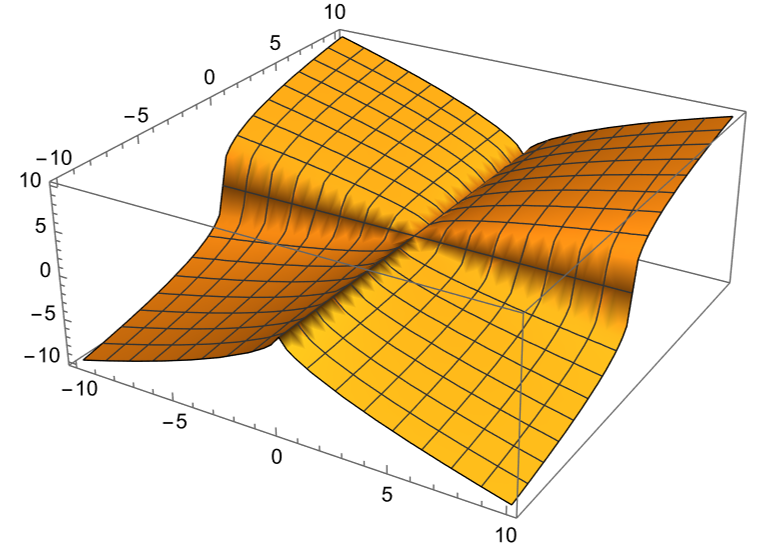
\includegraphics[width=0.4\textwidth]{img/ej10a.png}\\
                    Figura 2. Gráfico de $f(x,y)=\sqrt[3]{x^2y}$ con rectas contenidas.
                \end{center}
                Quizás una manera de visualizar la homogeneidad sea con las rectas de la Figura 2. Al fijar un $v$, por ejemplo el $(1,2)$, al ser multiplicado por un escalar me dará un múltiplo de $v$. Como $v\in\R^2$, la multiplicación por escalar me genera una recta en el plano $z=0$. Entonces si \[f(\alpha v)=\alpha f(v)\quad\forall v\in\R^2,\alpha\in\R\]
                al duplicar el vector $v$, se duplica su imagen, si lo triplico, la imagen también. Es decir, la imagen tiene un incremento constante. Esto se traduce a que la imagen de los puntos de una recta, son una recta. Y como esto sucede con todos los puntos de $\R^2$, se podría decir que la imagen es la unión de las rectas con parametrización:\[\sigma(t)=\left\{\begin{matrix}
                    at\\bt\\\sqrt[3]{(at)^2bt}
                \end{matrix}\right\}\quad a,b\text{ reales fijos},t\in[-\infty,\infty]\]
                En la Figura 3 se observan como un conjunto de estas rectas se aproxima a la función.
                \begin{center}
                    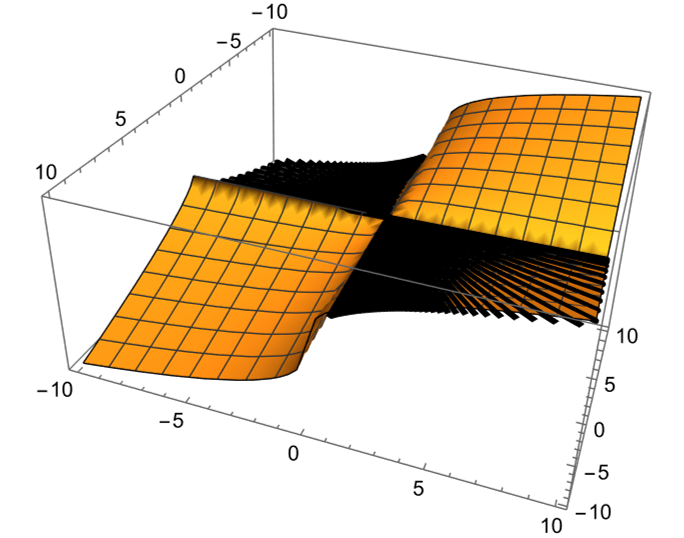
\includegraphics[width=0.4\textwidth]{img/ej10a2.png}\\
                    Figura 3. Gráfico de $f(x,y)=\sqrt[3]{x^2y}$ con múltiples rectas.
                \end{center}
            \end{mdframed}
        \item Dar un ejemplo de una función $g:\C\to\C$ tal que\[g(u+v)=g(u)+g(v)\quad\forall u,v\in\C\] pero que $g$ no sea lineal.
            \begin{mdframed}[style=s]
                La función del ejercicio 8d) cumple con esta condición. 
            \end{mdframed}
    \end{enumerate}
        \item \begin{enumerate}
        \item Sea $R_\alpha:\R^2\to\R^2$ la función que define la rotación en un ángulo $\alpha$ (fijo) en sentido antihorario, es decir \[R_\alpha(x,y)=(x \cos(\alpha)-y\sin(\alpha),x\sin(\alpha)+y\cos(\alpha))\quad\forall(x,y)\in\R^2\]
            \begin{enumerate}
                \item[1)] Probar que $R_\alpha$ es una transformación lineal para cualquier valor del ángulo $\alpha$ fijo.
                    \begin{mdframed}[style=s]
                        Sean $u,v\in\R^2,\lambda\in\R, u=(u_1,u_2),v=(v_1,v_2)$
                        \begin{align*}
                            T(u+v)&=T((u_1,u_2)+(v_1,v_2))\\
                            \text{Suma en }\R^2&=T(u_1+v_1,u_2+v_2)\\
                            \text{Definición T}&=((u_1+v_1)\cos(\alpha)-(u_2+v_2)\sin(\alpha),(u_1+v_1)\sin(\alpha)+(u_2+v_2)\cos(\alpha))\\
                            \text{Distributividad}&=(u_1\cos(\alpha)-u_2\sin(\alpha)+v_1\cos(\alpha)-v_2\sin(\alpha),\\
                            &\qquad u_1\sin(\alpha)+u_2\cos(\alpha)+v_1\sin(\alpha)+v_2\cos(\alpha))\\
                            \text{Suma en }\R^2&=(u_1\cos(\alpha)-u_2\sin(\alpha),u_1\sin(\alpha)+u_2\cos(\alpha))\\
                            &\qquad +(v_1\cos(\alpha)-v_2\sin(\alpha),v_1\sin(\alpha)+v_2\cos(\alpha))\\
                            \text{Definición T}&=T(u_1,u_2)+T(v_1,v_2)\\
                            &=T(u)+T(v)
                        \end{align*}
                        Por otra parte, sea $v=(v_1,v_2)\in\R^2,\lambda\in\R$
                        \begin{align*}
                            T(\lambda v)&=T(\lambda(v_1,v_2))\\
                            \text{Producto por escalar }\R^2&=T(\lambda v_1,\lambda v_2)\\
                            \text{Definición T}&=((\lambda v_1)\cos(\alpha)-(\lambda v_12)\sin(\alpha),(\lambda v_1)\sin(\alpha)+(\lambda v_2)\cos(\alpha))\\
                            \text{Factor común}&=\lambda(v_1\cos(\alpha)-v_2\sin(\alpha),v_1\sin(\alpha)+v_2\cos(\alpha))\\
                            \text{Definición T}&=\lambda T(v_1,v_2)\\
                            &=\lambda T(v)
                        \end{align*}
                        Por lo tanto, $T$ es una transformación lineal.
                    \end{mdframed}
                \item[2)] Determinar la imagen por $R_{\frac{\pi}{2}}$ de $P=(0,3),Q(3,1)$ y $S=(1,-1)$. Graficar el triángulo $PQS$ y su transformado en el mismo sistema de coordenadas.
                    \begin{mdframed}[style=s]
                        \[R_{\frac{\pi}{2}}(0,3)=(-3,0)\qquad R_{\frac{\pi}{2}}(3,1)=(-1,3)\qquad R_{\frac{\pi}{2}}(1,-1)=(1,1)\]
                        En la Figura 4 se puede ver como queda el triángulo transformado
                        \begin{center}
                            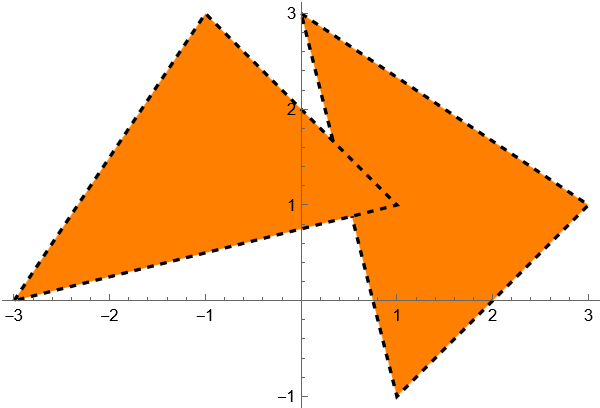
\includegraphics[width=0.4\textwidth]{img/ej11a.png}\\
                            Figura 4. Triángulo antes y después de ser transformado por $R_{\frac{\pi}{2}}$
                        \end{center}
                    \end{mdframed}
            \end{enumerate}
        \item Sea $S_Y:\R^2\to\R^2$ la función simetría respecto al eje $y$, es decir\[S_Y(x,y)=(-x,y)\quad\forall(x,y)\in\R^2.\]
            \begin{enumerate}
                \item[1)] Probar que $S_Y$ es una transformación lineal.\pagebreak
                    \begin{mdframed}[style=s]
                        Sean $u=(u_x,u_y),v=(v_x,v_y)\in\R^2,\alpha\in\R$
                        \begin{align*}
                            S_Y(\alpha u+v)&=S_Y(\alpha(u_x,u_y)+(v_x,v_y))\\
                            \text{Suma y prod por escalar}&=S_Y(\alpha u_x+v_x,\alpha u_y+v_y)\\
                            \text{Definición }S_Y&=(-(\alpha u_x+v_x),\alpha u_y+v_y)\\
                            \text{Suma en }\R^2&=(-\alpha u_x,\alpha u_y)+(-v_x,v_y)\\
                            \text{Prod por escalar}&=\alpha(-u_x,u_y)+(-v_x,v_y)\\
                            \text{Definición }S_Y&=\alpha S_Y(u_x,u_y)+S_Y(v_x,v_y)\\
                            &=\alpha S_Y(u)+S_Y(v)
                        \end{align*}
                    \end{mdframed}
                \item Determinar la imagen por $S_Y$ de $A=(0,1),B=(2,4),C=(4,3)$ y $D=(2,0)$. Graficar el rectángulo $ABCD$ y su transformado en el mismo sistema de coordenadas.
                    \begin{mdframed}[style=s]
                        \[S_Y(A)=(0,1)\qquad S_Y(B)=(-2,4)\qquad S_Y(C)=(-4,3)\qquad S_Y(D)=(-2,0)\qquad\]
                        En la Figura 5 se puede ver como queda el rectángulo transformado
                        \begin{center}
                            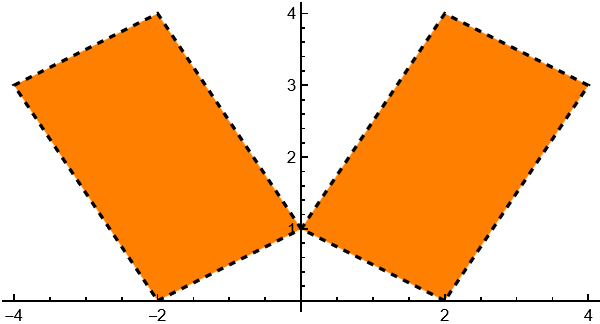
\includegraphics[width=0.4\textwidth]{img/ej11b.png}\\
                            Figura 5. Rectángulo antes y después de ser transformado por $S_Y$
                        \end{center}
                    \end{mdframed}
            \end{enumerate}
        \item Sea $H_k:\R^2\to\R^2$ la función homotecia de razón $k\in\R$ (fijo), es decir\[H_k(x,y)=(kx,ky)\quad\forall(x,y)\in\R^2.\]
            \begin{enumerate}
                \item[1)] Probar que $H_k$ es una transformación lineal para cualquier valor de $k\in\R$ fijo.
                    \begin{mdframed}[style=s]
                        Sean $u=(u_x,u_y),v=(v_x,v_y)\in\R^2,\alpha\in\R$
                        \begin{align*}
                            H_k(\alpha u+v)&=H_k(\alpha(u_x,u_y)+(v_x,v_y))\\
                            \text{Suma y prod por escalar}&=H_k(\alpha u_x+v_x,\alpha u_y+v_y)\\
                            \text{Definición }H_k&=(k(\alpha u_x+v_x),k(\alpha u_y+v_y))\\
                            \text{Suma en }\R^2&=(k\alpha u_x,k\alpha u_y)+(kv_x,kv_y)\\
                            \text{Prod por escalar}&=\alpha(ku_x,ku_y)+(kv_x,kv_y)\\
                            \text{Definición }H_k&=\alpha H_k(u_x,u_y)+H_k(v_x,v_y)\\
                            &=\alpha H_k(u)+H_k(v)
                        \end{align*}
                        Por lo tanto $H_k$ es una transformación lineal.
                    \end{mdframed}
                \item[2)] Determinar la imagen de $H_2$ de $A=(0,-1),B=(1,2)$ y $C=(3,1)$. Graficar el triángulo $ABC$ y su transformado en el mismo sistema de coordenadas.
                    \begin{mdframed}[style=s]
                        \[H_2(0,-1)=(0,-2)\qquad H_2(1,2)=(2,4)\qquad H_2(3,1)=(6,2)\]
                        En la Figura 6 se puede ver como queda el triángulo transformado
                        \begin{center}
                            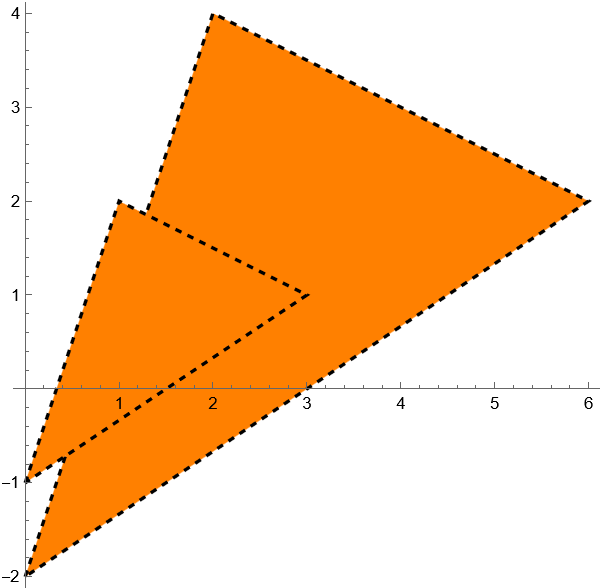
\includegraphics[width=0.4\textwidth]{img/ej11c.png}\\
                            Figura 6. Triángulo antes y después de ser transformado por $H_2$
                        \end{center}
                    \end{mdframed}
            \end{enumerate}
        \item Sea $P_X:\R^2\to\R^2$ la función proyección sobre el eje $x$.
            \begin{enumerate}
                \item[1)] Hallar una expresión analítica para $P_X$ y probar que es una transformación lineal.
                    \begin{mdframed}[style=s]
                        \[P_X(x,y)=(x,0)\]
                        Sean $u=(u_x,u_y),v=(v_x,v_y)\in\R^2,\alpha\in\R$
                        \begin{align*}
                            P_X(\alpha u+v)&=P_X(\alpha(u_x,u_y)+(v_x,v_y))\\
                            \text{Suma y prod por escalar}&=P_X(\alpha u_x+v_x,\alpha u_y+v_y)\\
                            \text{Definición }P_X&=(\alpha u_x+v_x,0)\\
                            \text{Suma en }\R^2&=(\alpha u_x,0)+(v_x,0)\\
                            \text{Prod por escalar}&=\alpha(u_x,0)+(kv_x,0)\\
                            \text{Definición }P_X&=\alpha P_X(u_x,u_y)+P_X(v_x,v_y)\\
                            &=\alpha P_X(u)+P_X(v)
                        \end{align*}
                        Por lo tanto, $P_X$ es una transformación lineal.
                    \end{mdframed}
                \item[2)] Determinar la imagen por $P_X$ de $A=(0,1),B=(2,4),C=(4,3)$ y $D=(2,0)$. Graficar el rectángulo $ABCD$ y su transformado, en el mismo sistema de coordenadas.
                    \begin{mdframed}[style=s]
                        \[P_X(0,1)=(0,0)\qquad P_X(2,4)=(2,0)\qquad P_X(4,3)=(4,0)\qquad P_X(2,0)=(2,0)\qquad \]
                        En la Figura 7 se puede ver como queda el rectángulo transformado
                        \begin{center}
                            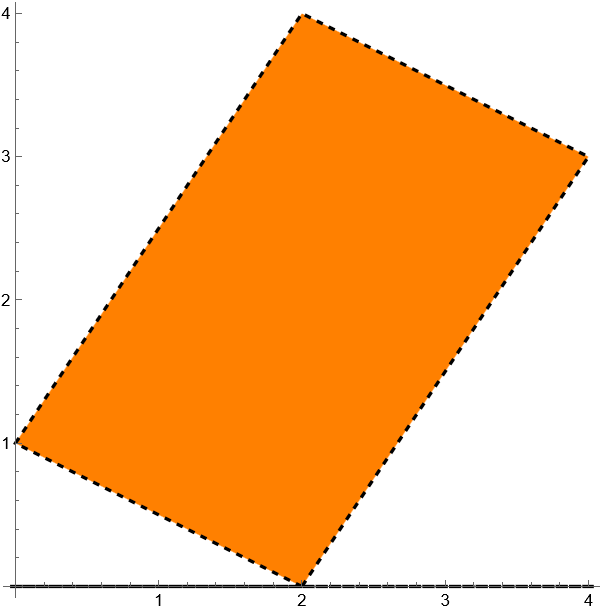
\includegraphics[width=0.4\textwidth]{img/ej11d.png}\\
                            Figura 7. Rectángulo antes y después de ser transformado por $P_X$
                        \end{center}
                    \end{mdframed}
            \end{enumerate}
    \end{enumerate}
        \item Se dice que una transformación $T:\R^n\to\R^n$ es una isometría si preserva distancias, es decir\[dist(P,Q)=dist(T(P),T(Q))\quad\forall P,Q\in\R^n.\] Analizar cuáles de las transformaciones del ejercicio anterior, son isometrías.
    \begin{mdframed}[style=s]
        Todas las transformaciones son de $\R^2$ en $\R^2$, la distancia está definida como \[dist(u,v)=\sqrt{u_xv_x+u_yv_y}\]
        \begin{enumerate}
            \item Sean $u,v\in\R^2,dist(R_\alpha(u),R_\alpha(v))=$
                \begin{align*}
                    &\text{\tiny(Definición $R_\alpha$)}\\
                    &=dist((u_x\cos(\alpha)-u_y\sin(\alpha),u_x\sin(\alpha)+u_y\cos(\alpha)),(v_x\cos(\alpha)-v_y\sin(\alpha),v_x\sin(\alpha)+v_y\cos(\alpha)))\\
                    &\text{\tiny(Definición dist)}\\
                    &=\sqrt{(u_x\cos(\alpha)-u_y\sin(\alpha))(v_x\cos(\alpha)-v_y\sin(\alpha))+(u_x\sin(\alpha)+u_y\cos(\alpha))(v_x\sin(\alpha)+v_y\cos(\alpha))}\\
                    &\text{\tiny(Distributividad y factor común)}\\
                    &=\sqrt{u_xv_x(\cos^2\alpha+\sin^2\alpha)+u_yv_y(\cos^2\alpha+\sin^2\alpha)}\\
                    &\text{\tiny($1=\cos^2\alpha+\sin^2\alpha$)}\\
                    &=\sqrt{u_xv_x+u_yv_y}\\
                    &\text{\tiny(Definición dist)}\\
                    &=dist(u,v)
                \end{align*}
                Por lo tanto, $R_\alpha$ es una isometría.
            \item Sean $u,v\in\R^2$
                \begin{align*}
                    dist(S_Y(u),S_Y(v))&=dist((-u_x,u_y),(-v_x,v_y))&&\text{Definición }S_Y\\
                    &=\sqrt{(-u_x)(-v_x)+u_yv_y}&&\text{Definición dist}\\
                    &=\sqrt{u_xv_x+u_yv_y}&&\text{Producto en }\R\\
                    &=dist(u,v)&&\text{Definición dist}
                \end{align*}
                Por lo tanto, $S_Y$ es una isometría.
            \item En la Figura 4, se ve que $H_2$ no es una isometría, pero a pesar de esto, la distancia tiene una peculiaridad:\\
                Sean $u,v\in\R$
                \begin{align*}
                    dist(H_2(u),H_2(v))&=dist((2u_x,2u_y),(2v_x,2v_y))\\
                    &=\sqrt{4u_xv_x+4u_yv_y}\\
                    &=2\sqrt{u_xv_x+u_yv_y}\\
                    &=2\cdot dist(u,v)
                \end{align*}
                La transformación $H_2$ duplica las distancias entre dos vectores cualesquiera.
            \item En la Figura 5, se ve que $P_X$ no es una isometría.
        \end{enumerate}
        \textbf{Aclaración:} La justificación gráfica sólo es válida en los casos en que no sea una isometría, ya que la definición especifíca que se debe cumplir para cualquier par de vectores, si encuentro un contraejemplo, ya es suficiente. Sin embargo, para probar que sí es una isometría, no me alcanza con ver que un conjunto (como los casos graficados en 11.a y 11.b) cumplan, ¿qué pasa si hay algún par de vectores en una región no contemplada que rompe la condición? No lo estaría teniendo en cuenta. Por eso, es necesario probar para dos vectores genéricos.
    \end{mdframed}
        \item \begin{enumerate}
        \item Probar que existe una única transformación lineal $T:\R^2\to\R^2$ tal que $T(1,1)=(-5,3)$ y $T(-1,1)=(5,2)$. Determinar $T(5,3)$ y $T(-1,2)$.
            \begin{mdframed}[style=s]
                $\R^2$: un $\R$-EV de dimensión 2. $B=\{(1,1),(-1,1)\}$ es base de $\R^2$ por ser dos vectores del espacio li. Además, ya que $(-5,3),(5,2)\in\R^2$, se cumplen las hipótesis del \textbf{Teorema 2.3}. Entonces, existe una única transformación lineal $T:\R^2\to\R^2$ tal que\[T(1,1)=(-5,3)\quad T(-1,1)=(5,2)\]Un vector $v=(x,y)\in\R^2$ puede ser escrito como combinación lineal de los elementos de la base $B$,
                \begin{align*}
                    (x,y)&=\psi(1,1)+\eta(-1,1)\\
                    (x,y)&=(\psi-\eta,\psi+\eta)\qquad\to\psi=\frac{x+y}{2}\quad\eta=\frac{y-x}{2}\\
                    \to T(x,y)&=\frac{x+y}{2} T(1,1)+\frac{y-x}{2} T(-1,1)\\
                    \to T(x,y)&=\frac{x+y}{2}(-5,3)+\frac{y-x}{2}(5,2)\\
                    \to T(x,y)&=\left(-5x,\frac{1}{2}x+\frac{5}{2}y\right)
                \end{align*}
                Por lo tanto,\[T(5,3)=(-25,10)\qquad T(-1,2)=\left(5,\frac{9}{2}\right)\]
            \end{mdframed}
        \item Determinar si existe una transformación lineal $T:\R^2\to\R^2$ tal que $T(1,1)=(2,6),T(-1,1)=(2,5)$ y $T(2,7)=(5,3)$.
            \begin{mdframed}[style=s]
                Si tomo las primeras dos transformaciones, tengo un caso análogo al inciso anterior.
                \begin{align*}
                    T(x,y)&=\alpha T(1,1)+\beta T(-1,1)\\
                    &=\alpha(2,6)+\beta(2,5)\\
                    &=(2\alpha+2\beta,6\alpha+5\beta)\\
                    \to T(x,y)&=\left(2y,\frac{1}{2}x+\frac{11}{2}y\right)
                \end{align*}
                Sin embargo\[T(2,7)=\left(14,\frac{79}{2}\right)\neq (5,3)\]
                Se podría pensar en probar otro par de transformaciones y luego verficar una tercera. Las condiciones las podemos plantear de la siguiente manera:\[1)Tv_1=w_1\qquad 2)Tv_2=w_2\qquad 3)Tv_3=w_3\]
                Cualquier combinación de 2 de los $v_i$ son linealmente independientes, con lo cual son base. De esto, se concluye que, la transformación que cumpla con las condiciones 1 y 2 es única. Ahora suponiendo que ésta no cumple con 3, no tiene sentido intentar buscar una transformación que cumpla por ejemplo, 2 y 3 y luego ver si se cumple 1. Ya que la única transformación que cumple 1 y 2, es la hallada en un primer intento. (Quizás se pueda formalizar la idea.)
            \end{mdframed}
    \end{enumerate}
    \end{enumerate}
    \textbf{Optativos}
    \begin{enumerate}
        \item Sea $V=\{p\in\Z_2[x]:gr(p)\leq3\}$.
    \begin{enumerate}
        \item Probar que $V$ es un $\Z_2$-subespacio vectorial de $\Z_2[x]$.
            \begin{mdframed}[style=s]
                
            \end{mdframed}
        \item Probar que $B_1=\{1,1+x,x^2,x^3+1\}$ y $B_2=\{1,1+x,1+x+x^2,x^3\}$ son bases de $V$.
            \begin{mdframed}[style=s]
                
            \end{mdframed}
        \item Hallar las coordenadas de $p=x+x^2+x^3$ en cada una de las bases del ítem anterior.
            \begin{mdframed}[style=s]
                
            \end{mdframed}
    \end{enumerate}
        \item Analizar si $T:\Z_2\times\Z_2\to\Z_2\times\Z_2$ dada por $T(a,b)=(a,b)\odot(0,1)$ (pensando a $\Z_2\times\Z_2$ como $\Z_2$-EV) es una transformación lineal, donde
    \begin{center}
        $(a,b)\odot(c,d)=(ac+bd,ad+bc+bd)\quad \text{para todo }(a,b),(c,d)\in\Z_2\times\Z_2$      
    \end{center}    
    \begin{mdframed}[style=s]
        
    \end{mdframed}
    \end{enumerate}
\end{document}